\chapter{SWD dataset}

The unique constraints of in-cabin monitoring and the specific 
requirements for steering wheel detection necessitated the development 
of a custom dataset. Existing datasets, such as KITTI and nuScenes, 
predominantly focus on external vehicle perception, capturing objects 
like cars, pedestrians, and road signs. These datasets are tailored 
for outdoor environments and often lack the spatial resolution, 
balance, and context required for confined in-cabin spaces. 
Furthermore, the irregular rotational degrees of freedom (DOF) in 
interior setups, along with occlusions and limited sensor viewpoints, 
further complicate the application of outdoor 3D detection models to 
in-cabin scenarios.

To address these limitations, a dataset specifically designed for 
steering wheel detection was developed, incorporating high-quality 3D 
point clouds and ground truth bounding boxes to capture the full 3DOF 
of the steering wheel’s location and orientation.

The diversity in subjects, poses, and conditions in this dataset 
provides a comprehensive foundation for training and evaluating 3D 
object detection models specifically for steering wheel estimation. 
The following sections outline the protocols used for recording, 
data extraction, and ground truthss.


\section{Recording Procedure}
To accurately capture the steering wheel's position across multiple 
configurations, a recording protocol is set up using a board with 
ArUco markers \cite{opencv_aruco_detection} centered on the steering wheel as shown in \cref{fig:demo_model}. 
ArUco board helps with determining position and orientation of 
the steering wheel in 3D space as ground turth. A positional reference card, 
similar to \cref{fig:reference_board}, was placed adjacent to the steering wheel, displaying 
16 distinct steering wheel orientations for standardized positioning. 

This approach allowed us to systematically record the steering wheel 
in various orientations, providing a comprehensive dataset for training 
and evaluating 3D object detection models focused on steering wheel 
estimation.

The video recordings were conducted using an Azure Kinect camera 
embedded in a car demo model as demonstrated in \cref{fig:demo_model}. 
This camera was positioned on the ceiling, slightly over the driver’s 
shoulder, and angled to capture the entire steering wheel. 

\begin{figure}[ht]
    \centering
    \begin{subfigure}[t]{0.45\textwidth}
        \centering
        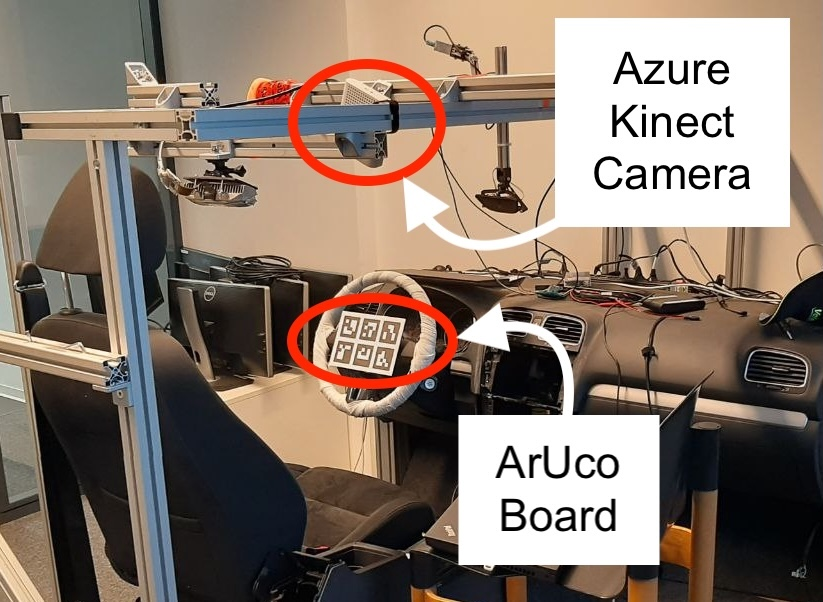
\includegraphics[width=\textwidth]{media/chapter 3/demo_model.jpg}
        \caption{ArUco board placed at the center of the steering wheel 
        and the Azure Kinect camera over the driver's shoulder 
        on the aluminium frames.}
        \label{fig:demo_model}
    \end{subfigure}\hfill
    \begin{subfigure}[t]{0.45\textwidth}
        \centering
        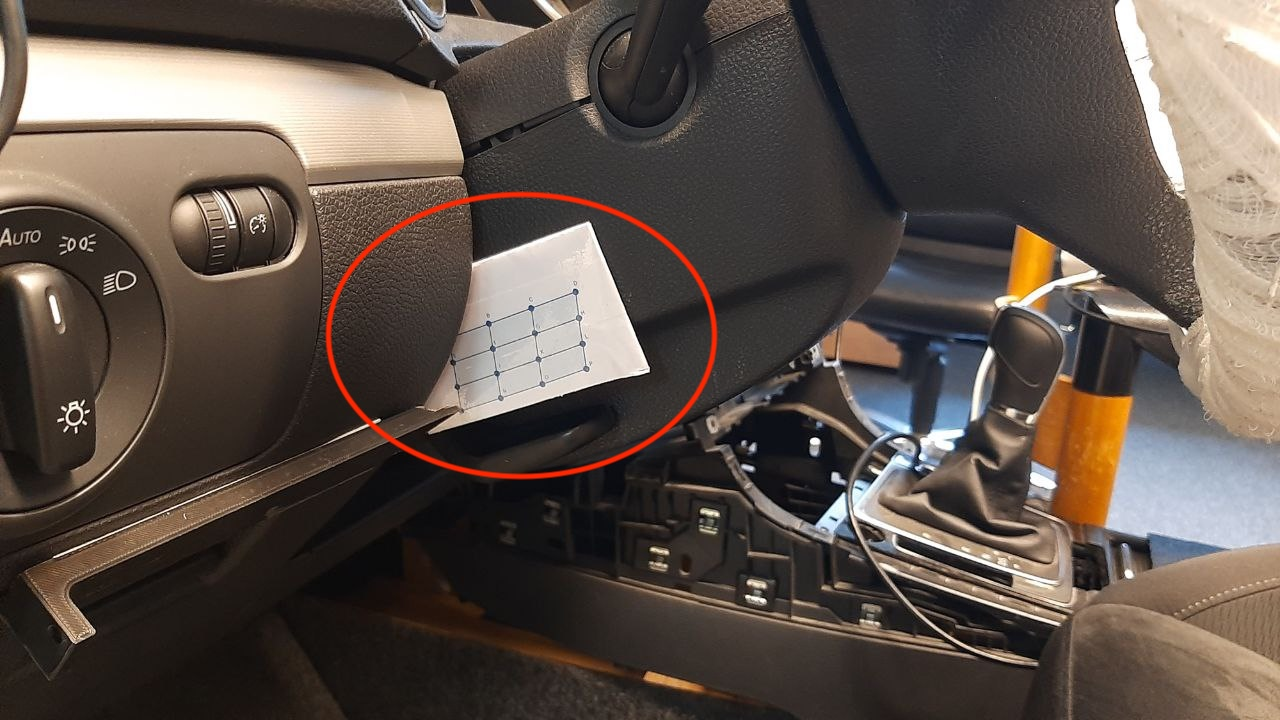
\includegraphics[width=\textwidth]{media/chapter 3/reference_board.jpg}
        \caption{A reference card was positioned next to the 
        steering wheel, illustrating 16 unique steering wheel orientations 
        to ensure standardized alignment.}
        \label{fig:reference_board}
    \end{subfigure}
    \caption{The demo model setup used for recording streams.}
\end{figure}

The dataset is composed of recordings from 10 unique participants, 
with each participant engaging with the steering wheel in 16 distinct 
posiitons. To introduce variability, the participants wore various 
accessories during the recordings. 
This resulted in a comprehensive dataset encompassing 72,747 training 
frames, 42,712 validation frames, and 29,099 testing frames. 
The steering wheel itself was covered with a white fabric to 
reduce reflections and enhance detection accuracy.

The dataset was recorded in two phases for each subject. 
First, a ground truth stream was captured with no driver 
present and the marker board fully visible as shown in \cref{fig:gt_stream}. 
This short footage was used to extract accurate ground truth data on 
the location and orientation of the steering wheel. 
Subsequently, a second stream was recorded with the driver 
interacting with the steering wheel, simulating a driving 
scenario. During these main recordings, the marker board was 
covered with a black surface as illustrated in \cref{fig:main_stream} to prevent unintended biases in 
the model training. 
The driver performed typical driving 
actions, such as steering with one or both hands, operating 
the dashboard, and other natural behaviors. 

For data processing, ground truths were extracted from the initial 
ground truth streams, while the main streams with the driver were 
used to extract point clouds for further experimentation.

\begin{figure}[ht]
    \centering
    \begin{subfigure}[t]{0.45\textwidth}
        \centering
        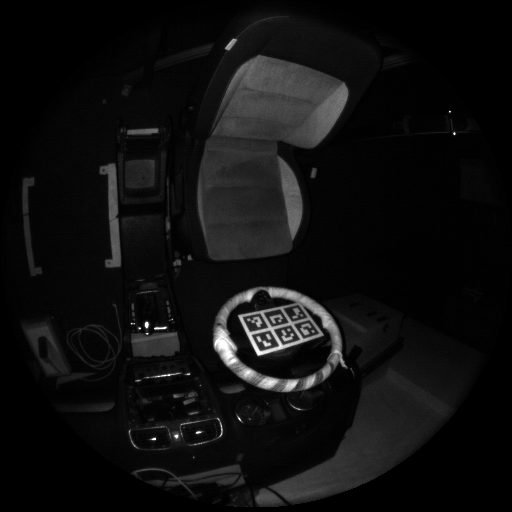
\includegraphics[width=\textwidth]{media/chapter 3/gt_stream.png}
        \caption{Ground truth data on the steering wheel’s 
        location and orientation were obtained from a stream 
        recorded without a driver, ensuring full visibility 
        of the marker board.}
        \label{fig:gt_stream}
    \end{subfigure}\hfill
    \begin{subfigure}[t]{0.45\textwidth}
        \centering
        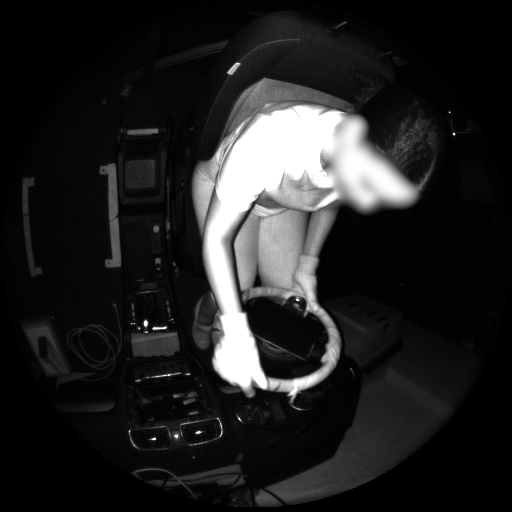
\includegraphics[width=\textwidth]{media/chapter 3/main_stream.png}
        \caption{A second stream was recorded with the driver 
        interacting with the steering wheel, simulating a 
        driving scenario, while the marker board was covered 
        to prevent biases in model training.}
        \label{fig:main_stream}
    \end{subfigure}
    \caption{Two stages of recording streams.}
\end{figure}

\section{Data Extraction}
In the initial data extraction phase, depth and amplitude 
information was derived from the video streams to create 
high-quality point clouds. The raw point clouds were then refined 
through a series of preprocessing steps to enhance their quality 
and suitability for accurate steering wheel position detection:

\begin{itemize}
    \item \textbf{Noise Reduction}: Filtering out extraneous points to 
    achieve a clear and uncluttered point cloud.
    \item \textbf{Distortion Correction}: Applied using 
    OpenCV's distortion matrices to enhance the clarity and accuracy 
    of both depth and amplitude images.
    \item \textbf{Edge Removal}: Points on the edges  
    were omitted due to their ambiguous positioning, which could 
    reduce the overall accuracy of the model.
    \item \textbf{Cropping}: The point cloud was cropped to a 
    50cm x 50cm x 50cm area around the steering wheel, ensuring that 
    the data was focused and relevant for model training and reducing 
    the dataset size.
\end{itemize}

These comprehensive preprocessing steps helped to create precise, 
refined point clouds that were well-suited for accurately detecting 
the position of the steering wheel.


\section{Ground Truth}
To generate ground truth data for the steering wheel's position and 
orientation, two approaches were explored due to the challenges presented by point sparsity and data distortion. The first approach, which involved annotating 2D points on images of the steering wheel and then mapping them to 3D space, failed to accurately represent the true position and orientation of the steering wheel. This was because the sparse and noisy distribution of the sampled points resulted in an imprecise oriented bounding box that did not capture the steering wheel's actual location and orientation with sufficient precision. 

In contrast, the second approach using ArUco board\cite{opencv_aruco_detection} proved to be a much more effective method. 
By first accurately estimating the 3D location of the ArUco markers and then fitting a plane to the markers' board, the precise location and orientation of the steering wheel were determined with three degrees of freedom. 
This method overcame the limitations of the initial approach and 
provided high-quality ground truth data that could be used for 
training and evaluating 3D object detection models.
Each approach will be discussed in more detail in the following sections.

In this dataset, the ground truth for each frame includes an 
oriented bounding box that represents the precise 3D position 
and orientation of the steering wheel. Bounding boxes are 
encoded as \([x, y, z, l, w, h, a_x, a_y, a_z]\), 
where \((x, y, z)\) represents the center of the bounding box, 
\((l, w, h)\) represents the dimensions of the box, 
\((a_x, a_y, a_z)\) represent the bounding box angle with 
the \(x\), \(y\), and \(z\) axes, respectively. 
\Cref{fig:sample_obbs} illustrates the ground truth data and oriented 
bounding boxes for sample point clouads from the dataset, 
providing a comprehensive visual representation of the 
steering wheel's 3D position and orientation.

\begin{figure}[ht]
    \centering
    \begin{subfigure}[t]{0.3\textwidth}
        \centering
        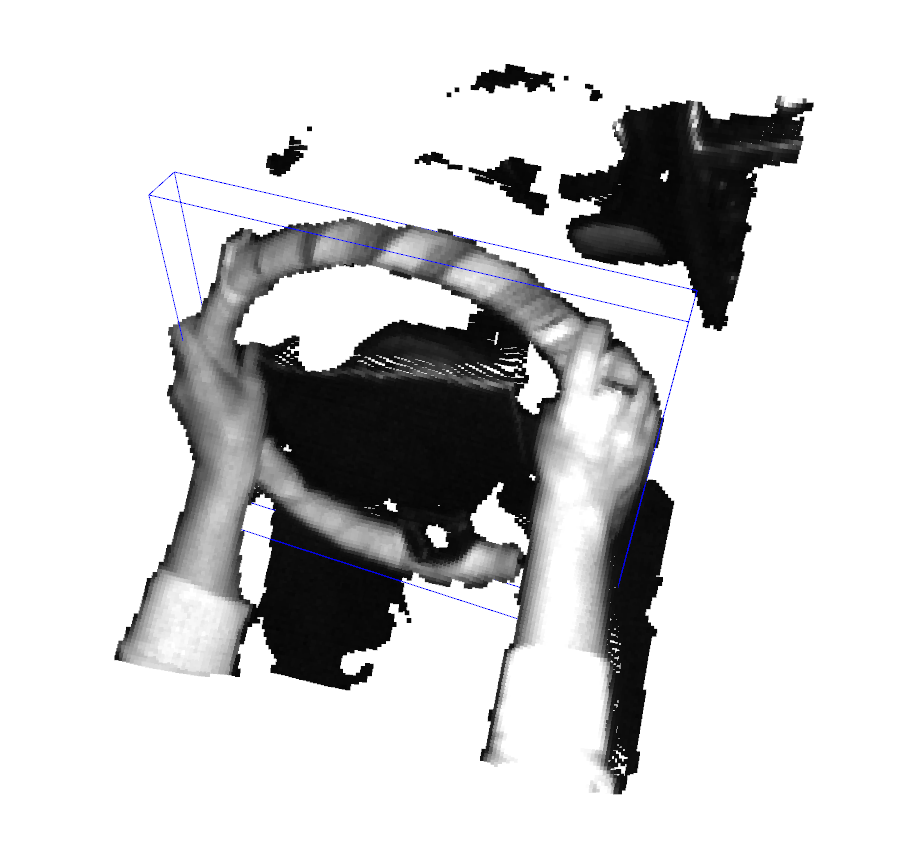
\includegraphics[width=\textwidth]{media/chapter 3/obb1.png}
    \end{subfigure}\hfill
    \begin{subfigure}[t]{0.3\textwidth}
        \centering
        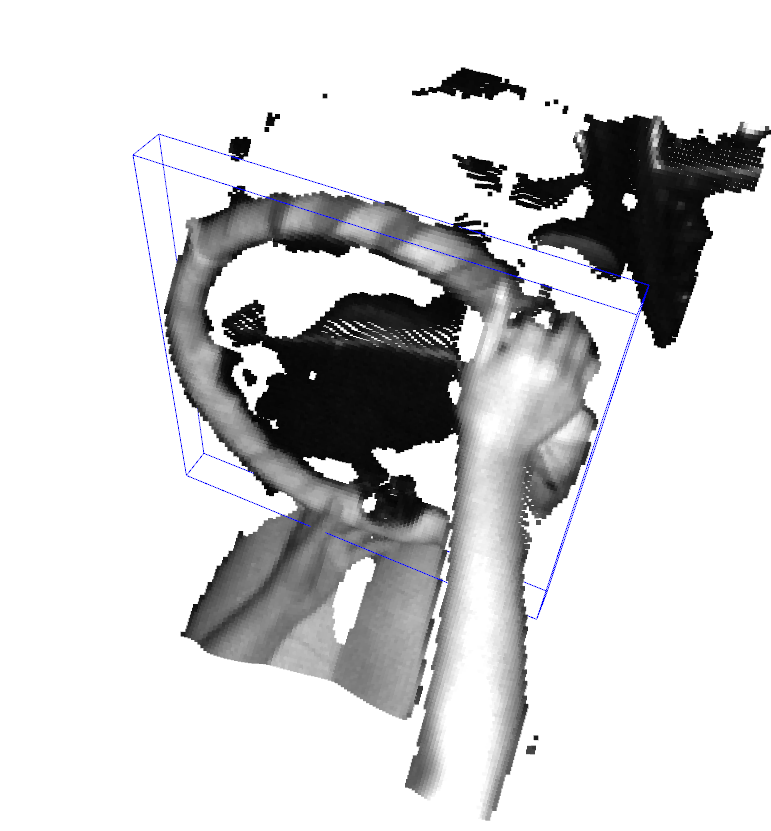
\includegraphics[width=\textwidth]{media/chapter 3/obb2.png}
    \end{subfigure}\hfill
    \begin{subfigure}[t]{0.3\textwidth}
        \centering
        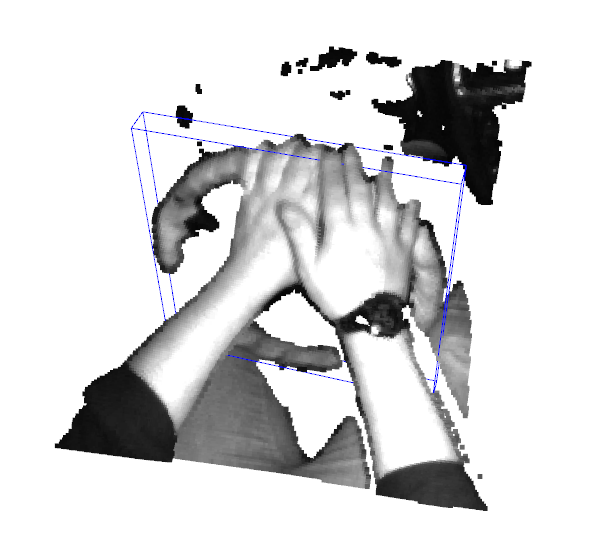
\includegraphics[width=\textwidth]{media/chapter 3/obb3.png}
    \end{subfigure}\\
    \begin{subfigure}[t]{0.3\textwidth}
        \centering
        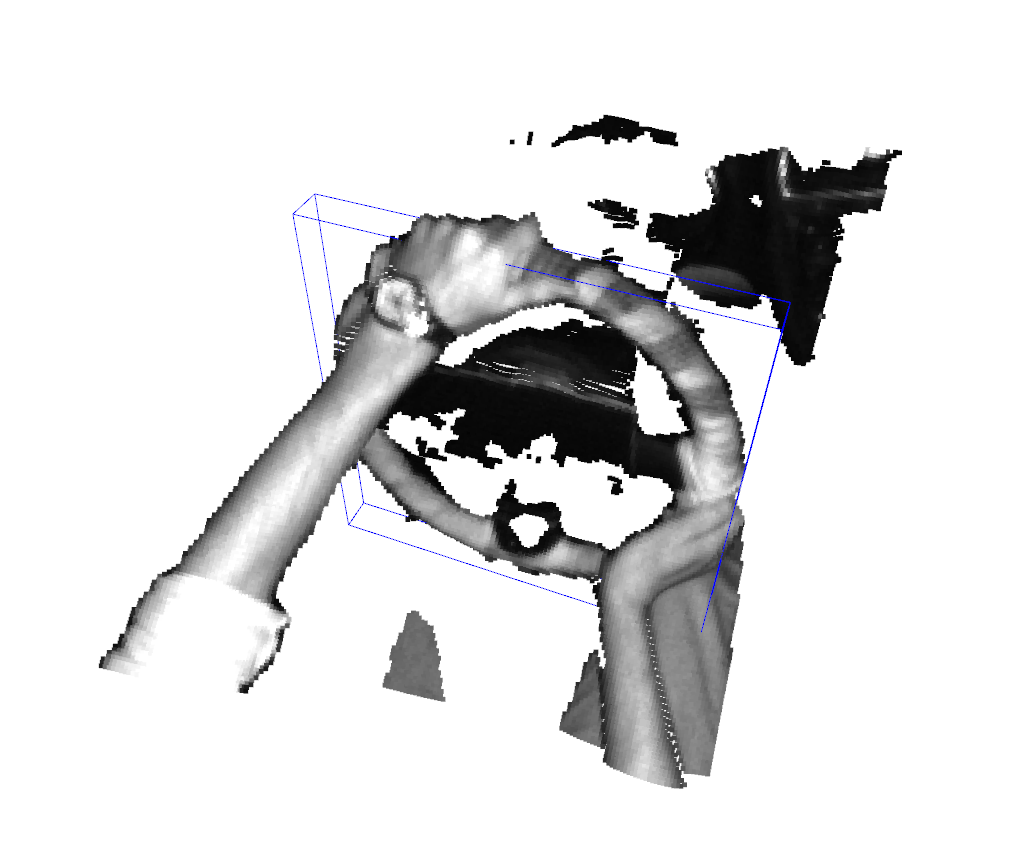
\includegraphics[width=\textwidth]{media/chapter 3/obb4.png}
    \end{subfigure}\hfill
    \begin{subfigure}[t]{0.3\textwidth}
        \centering
        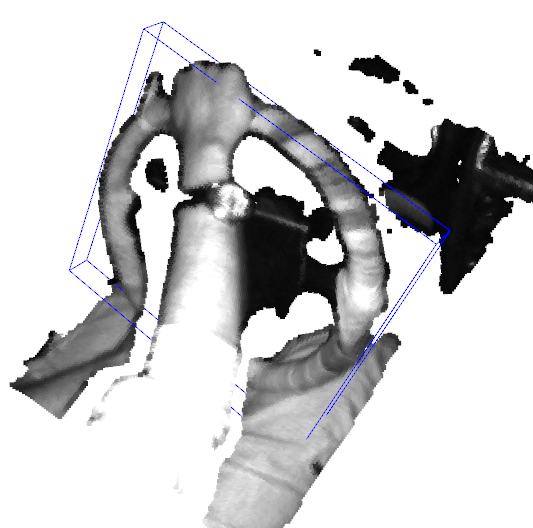
\includegraphics[width=\textwidth]{media/chapter 3/obb5.png}
    \end{subfigure}\hfill
    \begin{subfigure}[t]{0.3\textwidth}
        \centering
        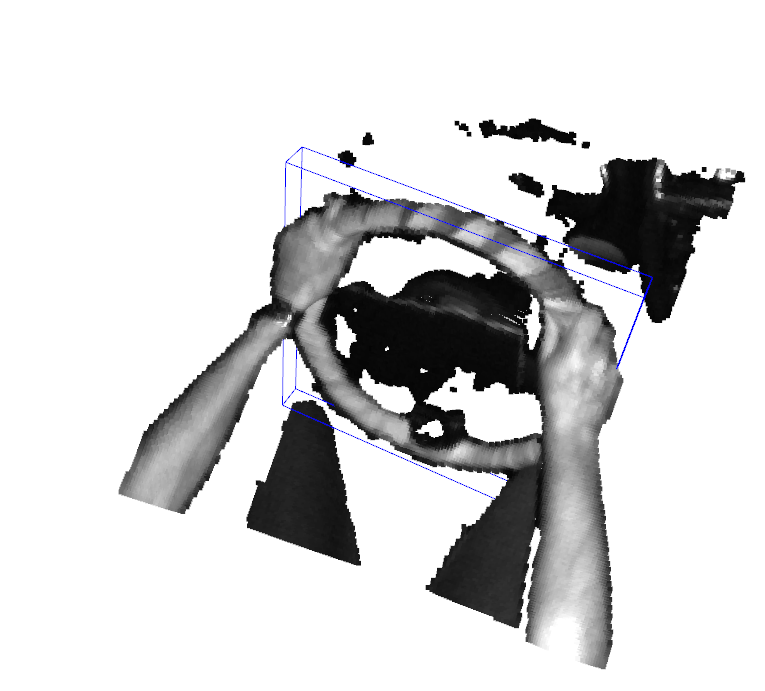
\includegraphics[width=\textwidth]{media/chapter 3/obb6.png}
    \end{subfigure}
    \caption{Oriented bounding boxes for sample point clouds from the dataset}
    \label{fig:sample_obbs}
\end{figure}


Given the ground truths, the steering wheel can be also represented 
by a torus shape, as depicted in \cref{fig:sample_toruses}. 
The torus shape can provide a more accurate geometric 
representation of the steering wheel, capturing its circular 
cross-section and three-dimensional nature more effectively 
than a bounding box. By modeling the steering wheel as a 
torus, its curvature and overall shape are captured more accurately, which is essential for accurate 3D pose estimation and 
object detection tasks.


\begin{figure}[ht]
    \centering
    \begin{subfigure}[t]{0.3\textwidth}
        \centering
        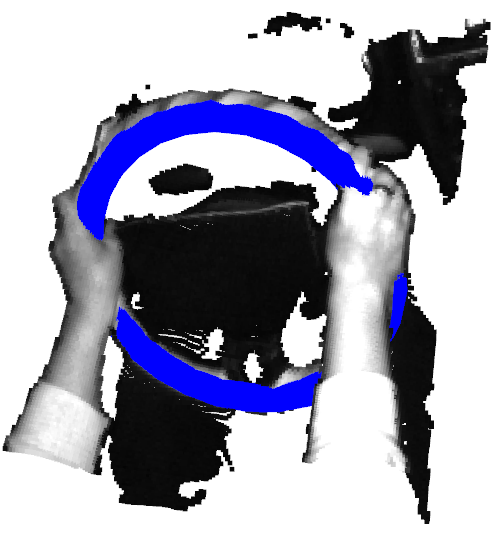
\includegraphics[width=\textwidth]{media/chapter 3/torus1.png}
    \end{subfigure}\hfill
    \begin{subfigure}[t]{0.3\textwidth}
        \centering
        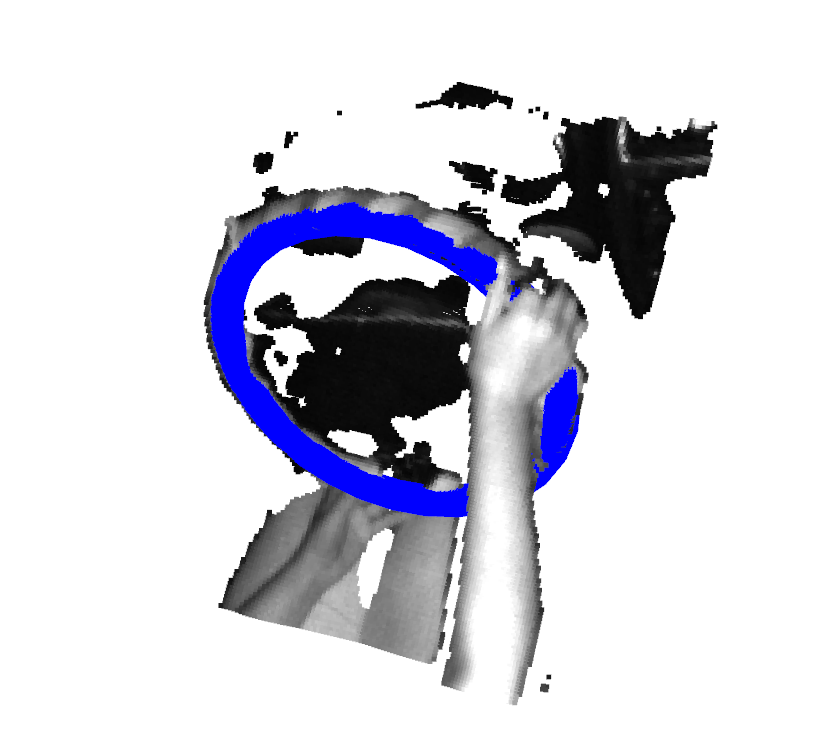
\includegraphics[width=\textwidth]{media/chapter 3/torus2.png}
    \end{subfigure}\hfill
    \begin{subfigure}[t]{0.3\textwidth}
        \centering
        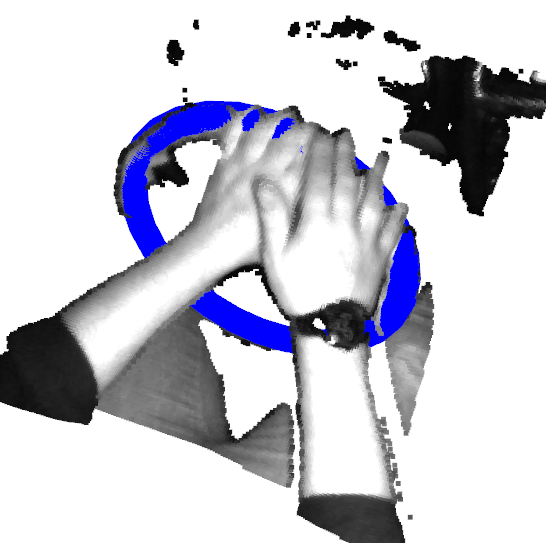
\includegraphics[width=\textwidth]{media/chapter 3/torus3.png}
    \end{subfigure}\\
    \begin{subfigure}[t]{0.3\textwidth}
        \centering
        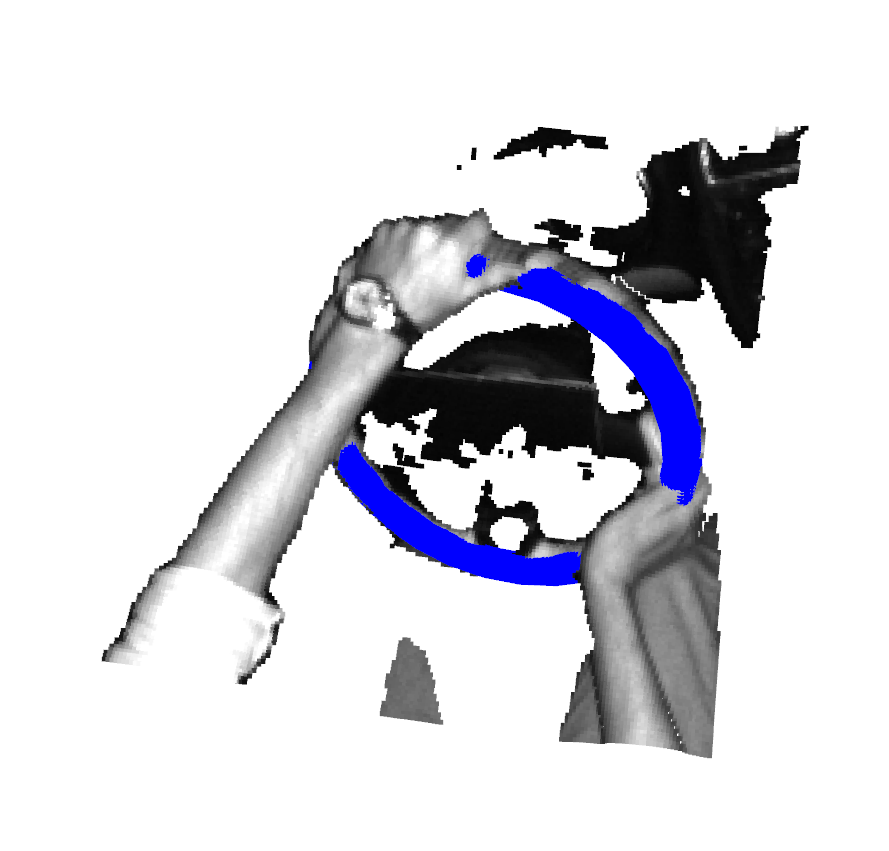
\includegraphics[width=\textwidth]{media/chapter 3/torus4.png}
    \end{subfigure}\hfill
    \begin{subfigure}[t]{0.3\textwidth}
        \centering
        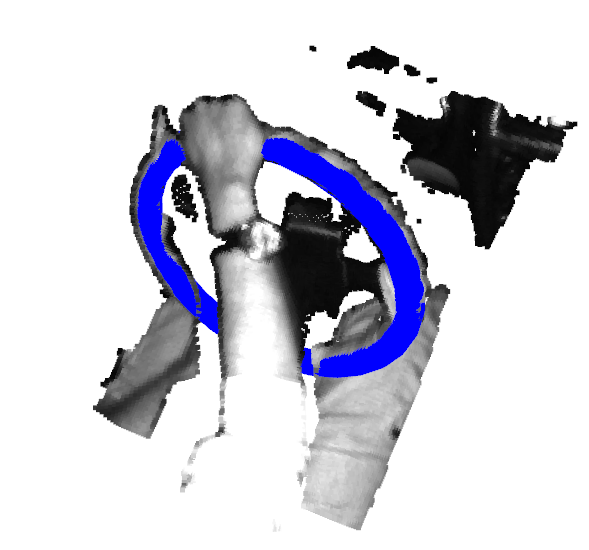
\includegraphics[width=\textwidth]{media/chapter 3/torus5.png}
    \end{subfigure}\hfill
    \begin{subfigure}[t]{0.3\textwidth}
        \centering
        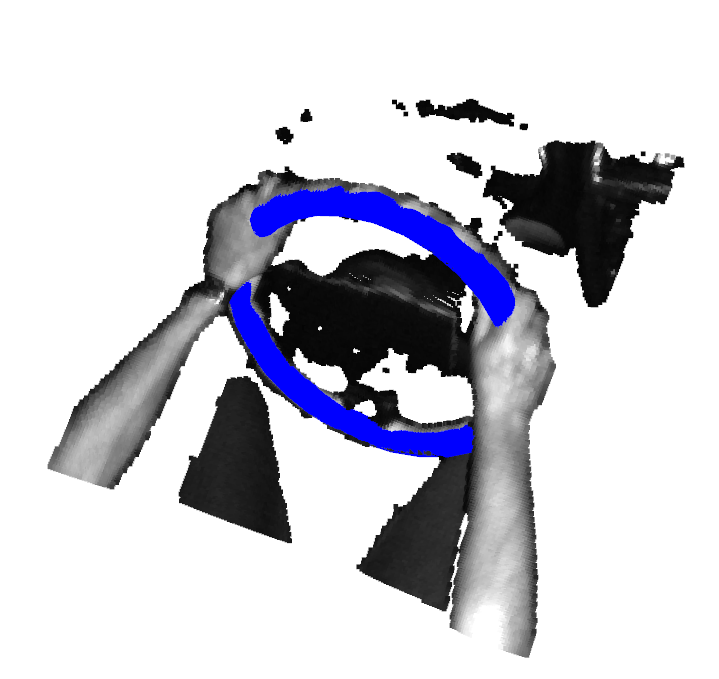
\includegraphics[width=\textwidth]{media/chapter 3/torus6.png}
    \end{subfigure}
    \caption{Torus representation of the steering wheel 
    for sample point clouds from the dataset}
    \label{fig:sample_toruses}
\end{figure}
